% Empirical section updated from frozen July 13 artifacts.
\section{Frozen July 13 empirical adjudication}
\label{sec:stable-results}

\begin{takeaway}
Proper full-law fit is not sufficient for the hardest new SID target.  Flexible
autoregressive and flow densities learn G8's static multimodal geometry extremely
well by held-out likelihood, but retain only 3--19\% of the held-out information
about its history-controlled mode weights and their samplers recover at most about
10\% of the corrected fourth-order effect.  A classifier-guided midpoint generator
raises EDM's median effect slope from 0.010 to 0.398 but remains badly attenuated,
and explicit endpoint experts reach only 0.336.  These interventions separate
missing global mass from missing fourth-order generator geometry.  In contrast, a balanced finite
classifier trained on the declared perturbation reaches Bayes AUC and 1--3\%
typed-effect error.  Across the wider suite, direct ratios are the most reliable
clean tangent route, while diffusion's accurate noisy response score frequently
fails to transfer to an accurate history tangent.  The data therefore isolate an
objective/estimand mismatch, not simply insufficient signal or an unstable sampler.
\end{takeaway}

\subsection{Frozen design and validation}

The core run crossed eight exact generators, all applicable models, two generator
seeds, two data seeds, and two model seeds.  All 784 expected cells completed; all
784 case records were valid; there were zero case failures and zero metric
failures.  The run used 8,000 training examples, a fixed 1,600-case validation
set, 512 test cases, one CPU thread, and one job at a time.  The eight crossed
cells per generator--model pair measure data and initialization variability, but
there are only two independent generated systems.  Consequently all intervals in
this subsection are developmental paired-bootstrap summaries, not confirmatory
system-level inference.

The evaluation contract keeps five endpoints distinct:
\begin{enumerate}
  \item fair energy score for conditional samples;
  \item NLL only for models with an exact normalized density;
  \item clean history-tangent NRMSE for direct normalized or ratio routes;
  \item noisy response-score NRMSE at standardized corruption $0.12$;
  \item noisy history-tangent NRMSE for diffusion, separated by its centering
  route.
\end{enumerate}
The zero-tangent estimator has NRMSE one.  The frozen bounded-energy numerical
rows are retained for audit but excluded from the primary fair-energy ranking
because that run used dependent finite-pool SIR.  The implementation has since
been replaced by exact i.i.d. rejection sampling with proposal caps and acceptance
diagnostics; this repairs future evaluation but does not retroactively change the
frozen table.

\subsection{Predictive-law fit: real flexibility gains, but metric-dependent}

Table~\ref{tab:law-winners} gives the best eligible route under the two common law
metrics.  Energy values are mean paired percentage changes from Gaussian NLL;
NLL values are paired nats per response vector.  Negative is better.

\begin{center}
\begin{tabularx}{\linewidth}{@{}l X r X r@{}}
\toprule
Law & Best fair-energy route & Change & Best exact-density route & NLL change \\
\midrule
G1 Gaussian sanity & Gaussian-anchored EDM & $-0.41\%$ & autoregressive MDN & $-0.118$ \\
G2 covariance & autoregressive MDN & $-0.66\%$ & autoregressive MDN & $-0.227$ \\
G3 matched skew & autoregressive MDN & $-0.44\%$ & autoregressive MDN & $-0.665$ \\
G4 separated modes & autoregressive MDN & $-2.25\%$ & autoregressive MDN & $-2.556$ \\
G5 near manifold & autoregressive Transformer & $-4.98\%$ & autoregressive Transformer & $-24.336$ \\
G6 rough history & Gaussian NLL & $0.00\%$ & Gaussian NLL & $0.000$ \\
G7 concentrated support & flow matching & $-1.18\%$ & autoregressive MDN & $-1.228$ \\
G8 functional shape & affine flow & $-1.89\%$ & autoregressive Transformer & $-18.343$ \\
\bottomrule
\end{tabularx}
\captionof{table}{Best eligible law-fit routes in the frozen core panel.}
\label{tab:law-winners}
\end{center}

\begin{figure}[ht]
\centering
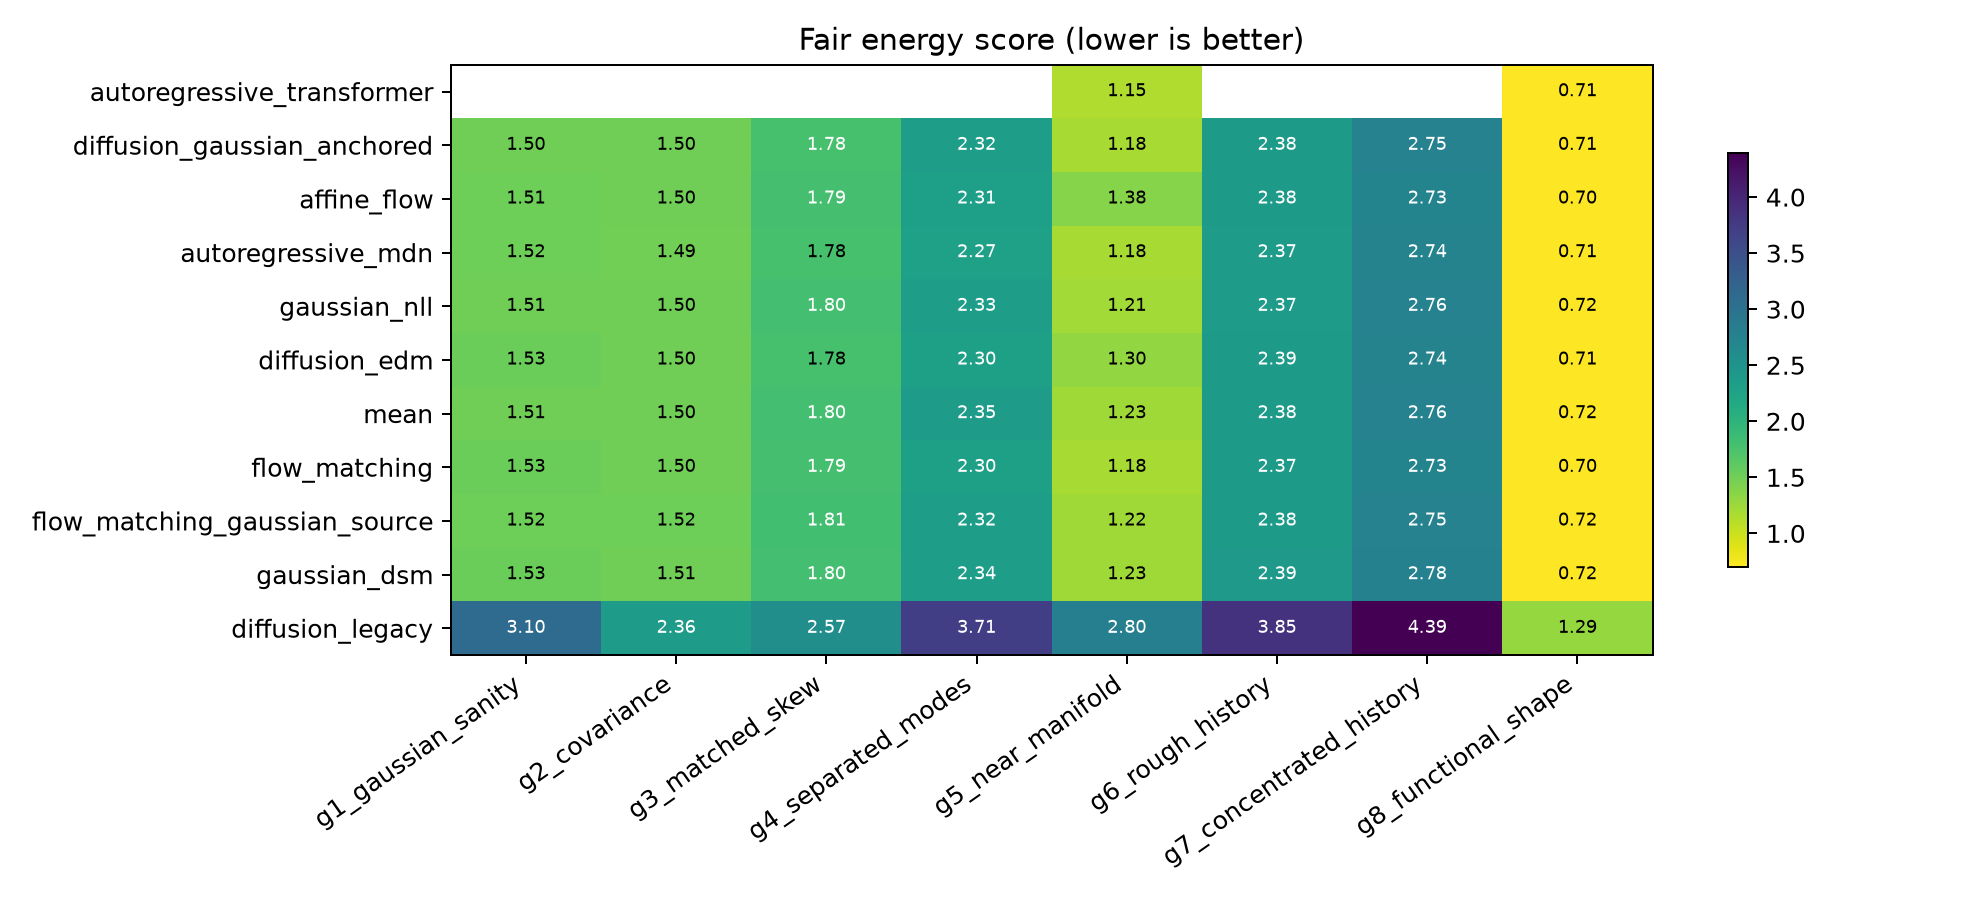
\includegraphics[width=\linewidth]{../../analysis/stable_sid_adjudication_2026-07-13-v2/core_energy_score.png}
\caption{Frozen fair-energy medians.  The bounded-energy row is excluded because
that run's SIR sampler did not provide i.i.d. draws.  Absolute scores should be
compared within a generator, not across response dimensions.}
\label{fig:stable-energy}
\end{figure}

Three conclusions are important.  First, the flexible normalized models clearly
learn non-Gaussian structure: relative to Gaussian, paired NLL improves in every
cell by about 2.56 nats on G4, 24.34 on G5, and 18.34 on G8 for the winning
models.  Second, fair energy sees only small improvements on G4/G7/G8 and can
therefore understate the value of fitting mode topology.  Third, likelihood and
sample geometry can disagree: on G5 the affine flow improves NLL by 23.24 nats
but makes energy score 14.0\% worse.  Neither metric alone is a sufficient SID
gate.

The stabilized EDM sampler is not a universal law winner.  Relative to Gaussian
its mean paired energy changes are $-1.78\%$ on G4, $-0.93\%$ on G7, and
$-1.42\%$ on G8, but $+6.03\%$ on G5 and $+1.37\%$ on G1.  Gaussian anchoring
repairs much of the G5 loss ($-3.25\%$ versus Gaussian), but the autoregressive
Transformer remains better ($-4.98\%$).  The legacy diffusion sampler is
43--130\% worse than Gaussian across the suite despite often having the best
noisy response-score estimate.  Stabilization therefore repairs generation, not
automatically derivative access.

The exact-rejection reevaluation closes the bounded-energy validity gap.  All 64
frozen checkpoints complete with i.i.d. draws; median acceptance ranges from
0.136 to 0.431, and the largest realized proposal tensor contains 4,092 proposals
under a 4,096 cap.  Exact fair-energy medians for G1--G8 are respectively
1.507, 1.504, 1.775, 2.301, 1.209, 2.382, 2.778, and 0.715.  These are competitive
with Gaussian and flow on several laws, but still trail the strongest flexible
frozen baseline on G4/G5/G7/G8.  More decisively, the exact G8 quartic NRMSE is
1.000 with slope $-0.00008$.  Exact sampling repairs the proper-score contract;
it does not repair the contrast objective.

\subsection{Clean SID: the ratio route wins most often, with sharp failures}

\begin{center}
\begin{tabularx}{\linewidth}{@{}l X r X@{}}
\toprule
Law & Best clean tangent route & Median NRMSE & Validity interpretation \\
\midrule
G1 Gaussian sanity & ratio critic & 0.532 & valid in all eight cells \\
G2 covariance & ratio critic & 0.582 & valid in all eight cells \\
G3 matched skew & ratio critic & 1.456 & no route beats zero \\
G4 separated modes & ratio critic & 0.424 & only reliable route \\
G5 near manifold & ratio critic & 0.585 & Transformer second at 0.881 \\
G6 rough history & ratio critic & 0.658 & all direct routes beat zero \\
G7 concentrated support & ratio critic & 1.604 & no route beats zero \\
G8 functional shape & autoregressive Transformer & 0.529 & ratio critic second at 0.616 \\
\bottomrule
\end{tabularx}
\captionof{table}{Clean history-tangent NRMSE; the zero estimator is one.}
\label{tab:clean-tangent-winners}
\end{center}

\begin{figure}[ht]
\centering
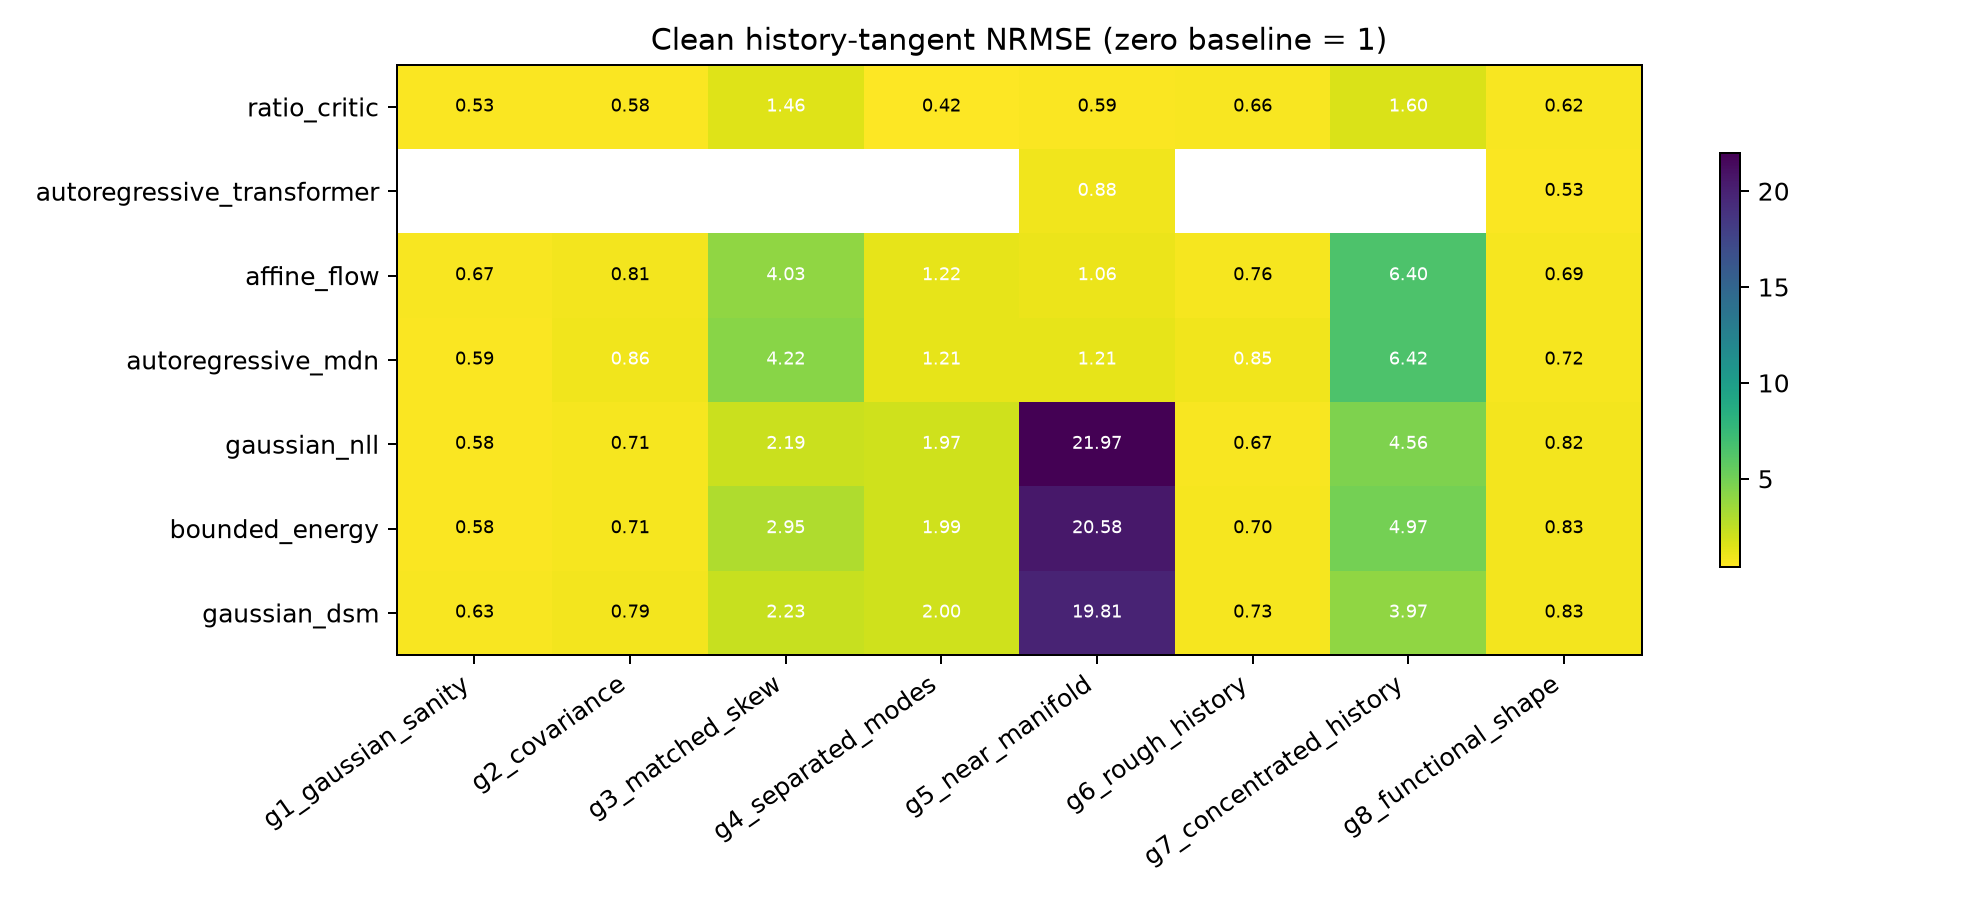
\includegraphics[width=\linewidth]{../../analysis/stable_sid_adjudication_2026-07-13-v2/core_clean_tangent_nrmse.png}
\caption{Clean history-tangent NRMSE with estimand and centering route held fixed.
Values above one lose to the zero-tangent estimator.}
\label{fig:stable-clean-tangent}
\end{figure}

This is the strongest empirical support for the SID-driven framing.  A direct
ratio critic is the clean-tangent winner on six of eight laws and is particularly
strong for separated mode occupancy (0.424) and the near-manifold mixture
(0.585), where the Gaussian tangent is unusable (1.97 and 21.97).  The normalized
Transformer wins G8 (0.529).  However, the ratio route is not a universal cure:
G3 skew and G7 concentrated support remain invalid at 1.456 and 1.604.  On the
one-sided finite log-ratio metric, every existing G8 route is invalid: ratio critic
1.066, Transformer 1.071, affine flow 1.086, and Gaussian 1.134.  Thus the law is
learnable while the declared finite adaptation is not yet reliable.

\subsection{Diffusion: response score and history SID empirically decouple}

The legacy diffusion has the lowest noisy response-score NRMSE on every generator
(0.216--0.753), yet after implementable model-sample centering its history-tangent
NRMSE is invalid on G3, G4, G5, and G7.  The corresponding medians are 2.390,
1.166, 1.125, and 5.852.  EDM and Gaussian-anchored EDM generally have better
samplers but worse mixed-history derivatives; on G8 their model-centered tangent
NRMSEs are 1.246 and 0.850 versus 0.631 for legacy diffusion.  This reverses their
sample-quality ordering.

An independent five-system invalidity replication reaches the same
location-versus-shape conclusion.  Averaging three fixed Transformer coordinate
orders, Transformer/diffusion tangent NRMSE is 0.497/0.751 on G1 location and
0.636/0.745 on G6 rough location, but 1.272/1.480 on G2 covariance,
1.014/3.852 on G3 skew, and 1.065/1.030 on G4 occupancy.  The oracle clean-to-noisy
gap is below 0.018, so small corruption does not explain the failure.  A
data-only history-Hyv\"arinen penalty also failed its frozen G2--G4 gate.  These
replications rule out the explanation that the core result is only one unlucky
initialization or one EDM implementation choice.

In a separate 64-dimensional G5 development system, the converged Transformer
has energy 1.1768, EDM 1.3226 (12.4\% worse), and legacy diffusion 1.7072
(45.1\% worse).  Diffusion generates samples roughly 250 times faster, so it has
a genuine computational advantage but no demonstrated quality advantage in that
system.

\subsection{Finite typed contrasts}

The frozen finite panel uses the exact same source/checkpoint snapshot, three
perturbation scales $\delta\in\{0.05,0.12,0.25\}$, and clean/noisy response laws.
Its complete manifest contains 212,832 valid metric rows, 4,704 diagnostic rows,
eight generators, 14 predictive-source labels, and seven finite routes; no metric
row failed.  The learned cells cross the same two generator, two data, and two
model seeds as the core panel.  One adapter seed is used, so these are exploratory
medians rather than adapter-robust confidence intervals.

At the primary clean scale $\delta=0.12$, the best learned typed-channel routes
are:

\begin{center}
\begin{tabularx}{\linewidth}{@{}l X r X@{}}
\toprule
Law & Best route/source & NRMSE & Interpretation \\
\midrule
G1 location & coupled samples, anchored EDM & 0.327 & clear recovery \\
G2 covariance & coupled samples, flow matching & 0.417 & clear recovery \\
G3 matched skew & signed Riesz, legacy diffusion & 1.003 & no valid route at this scale \\
G4 separated modes & central log ratio, MDN & 0.442 & clear recovery \\
G5 near manifold & central log ratio, ratio critic & 0.492 & clear recovery \\
G6 rough history & coupled samples, flow matching & 0.477 & clear recovery \\
G7 concentrated support & coupled samples, flow matching & 0.656 & useful but variable \\
G8 functional shape & coupled samples, Gaussian-source flow & 0.988 & cubic dictionary is blind \\
\bottomrule
\end{tabularx}
\end{center}

This is more favorable to sampler backends than the infinitesimal-tangent panel.
Direct common-random-number sample moments let flow or stabilized diffusion lead
G1, G2, G6, and G7; normalized or direct ratios lead G4 and G5.  Full-witness
reconstruction remains harder.  The best witness NRMSEs are 0.508 (G1), 0.651
(G2), 0.342 (G4), 0.639 (G5), 0.724 (G6), and 0.698 (G7), while G3 and G8 remain
approximately the zero witness.  The signed Riesz dictionary is generally
unstable and should not advance in its present form.

Perturbation scale is scientifically material.  At $\delta=0.25$, direct EDM
samples recover the G3 typed skew channel at NRMSE 0.660 versus an oracle-sample
Monte Carlo floor of 0.430; at $\delta=0.12$ the same clean route is 1.042.  At
the noisy $\sigma=0.12$ law and $\delta=0.12$, EDM reaches 0.727.  This is a real
home-field hint for stabilized generative sampling, but it does not establish
clean infinitesimal skew recovery: increasing $\delta$ changes the estimand, and
response noising changes the law.  More generally G4--G7 improve as the supported
contrast grows, reinforcing the finite rather than infinitesimal formulation.

The process returned nonzero only after atomically writing the complete artifacts,
when a post-write disk guard measured 3.87 GiB free against a 4.00 GiB floor.  The
manifest status, row counts, finiteness, and hashes were independently verified;
the resource event is retained in the audit rather than relabeled as a scientific
failure.

The G8 conclusion requires the analytically necessary fourth-order motif and exact
frame-occupancy readouts.  The current fixed response dictionary ends at cubic
order and is a predeclared negative-control limitation rather than evidence that
G8 has no signal.

The omitted target is not weak.  For generator seeds 61 and 67, the analytic
quartic constants are $D=8.619$ and $7.583$.  At control zero the exact central
quartic effects are 5.170/4.548 at $\delta=0.05$, 5.162/4.542 at
$\delta=0.12$, and 5.133/4.516 at $\delta=0.25$.  A 25,000-draw-per-side oracle
check at $\delta=0.12$ recovers both effects within 0.78 Monte Carlo standard
errors, while linear and quadratic motif contrasts stay near zero.  Hence a
learned method that misses the corrected quartic channel is missing a strong,
exactly identified higher-order effect; a cubic dictionary simply never asked the
right question.

A corrected frozen-checkpoint sample evaluation then asks that question directly.
It covers 96 records with 12 histories and 512 draws per side for every eligible
model; the oracle uses 2,048.  The oracle quartic NRMSE is 0.117 and its median
effect-calibration slope is 0.984.  Every learned sampler is essentially the zero
effect estimator:
\begin{center}
\begin{tabular}{@{}lrr@{}}
\toprule
Backend & Quartic NRMSE & Effect slope \\
\midrule
autoregressive MDN & 0.946 & 0.060 \\
affine flow & 0.949 & 0.051 \\
EDM & 0.994 & 0.006 \\
autoregressive Transformer & 0.994 & 0.007 \\
ordinary flow matching & 0.999 & 0.001 \\
Gaussian NLL & 1.000 & 0.000 \\
\bottomrule
\end{tabular}
\end{center}
Thus the large G8 likelihood gains come from learning the static multimodal path
geometry, while the backends recover only 0--6\% of its history-controlled
fourth-order effect.  This refines the diagnosis again: the original readout was
blind, and the fitted predictive laws use too little of their capacity for the
history-controlled mass change.  A continuously varying history with one response
per history could have contributed, so a separate factorial tests that hypothesis
directly.

That 48-cell factorial crosses two independent systems, two model seeds, a
balanced binary control, and a fixed-budget paired design with four outcomes per
state/control cell.  Binary randomization improves the strongest slope only to
$9.5\%$; fixed-budget pairing does not rescue it:

\begin{center}
\begin{tabular}{@{}lrr@{}}
\toprule
Backend & Unpaired binary slope & Paired/replicated slope \\
\midrule
autoregressive MDN & 0.095 & 0.082 \\
affine flow & 0.046 & 0.050 \\
autoregressive Transformer & 0.049 & 0.024 \\
EDM & 0.013 & 0.016 \\
flow matching & 0.001 & $-0.001$ \\
Gaussian NLL & 0.000 & 0.000 \\
\bottomrule
\end{tabular}
\end{center}

All 48 fits completed without failure.  The paired lane holds total training
rows at 8,000, so its additional within-state replication trades off against the
number of unique states; it rules out that fixed-budget repair, not every possible
replication regime.  More importantly, the shape control is state-independent in
G8, so persistent attenuation after a large supported $-1$ versus $+1$ contrast
points toward objective/representation allocation rather than local support or a
weak perturbation.

An exact noise-scale audit isolates why denoising is especially vulnerable on
this law.  Across four independent G8 systems and 5,000 exact draws per control
side and system, the clean $+1$ versus $-1$ laws retain median
Jensen--Shannon divergence $0.151$ nats and Bayes AUC $0.770$.  Their response
scores differ by only $3.86\%$ of the score RMS, while the history-tangent RMS is
$0.595$.  Noising initially exposes the inter-frame ambiguity region: relative
response-score separation peaks at $13.56\%$ near $\sigma=0.20$.  But at that
same scale Jensen--Shannon divergence has already fallen to $0.0887$ nats.  By
$\sigma=0.60$, divergence is $0.00195$ nats and history-tangent RMS is $0.0670$.
Thus the DSM signal has a narrow intermediate-noise window; ordinary averaging
over noise levels is poorly aligned with preservation of the finite SID target.

\begin{figure}[ht]
\centering
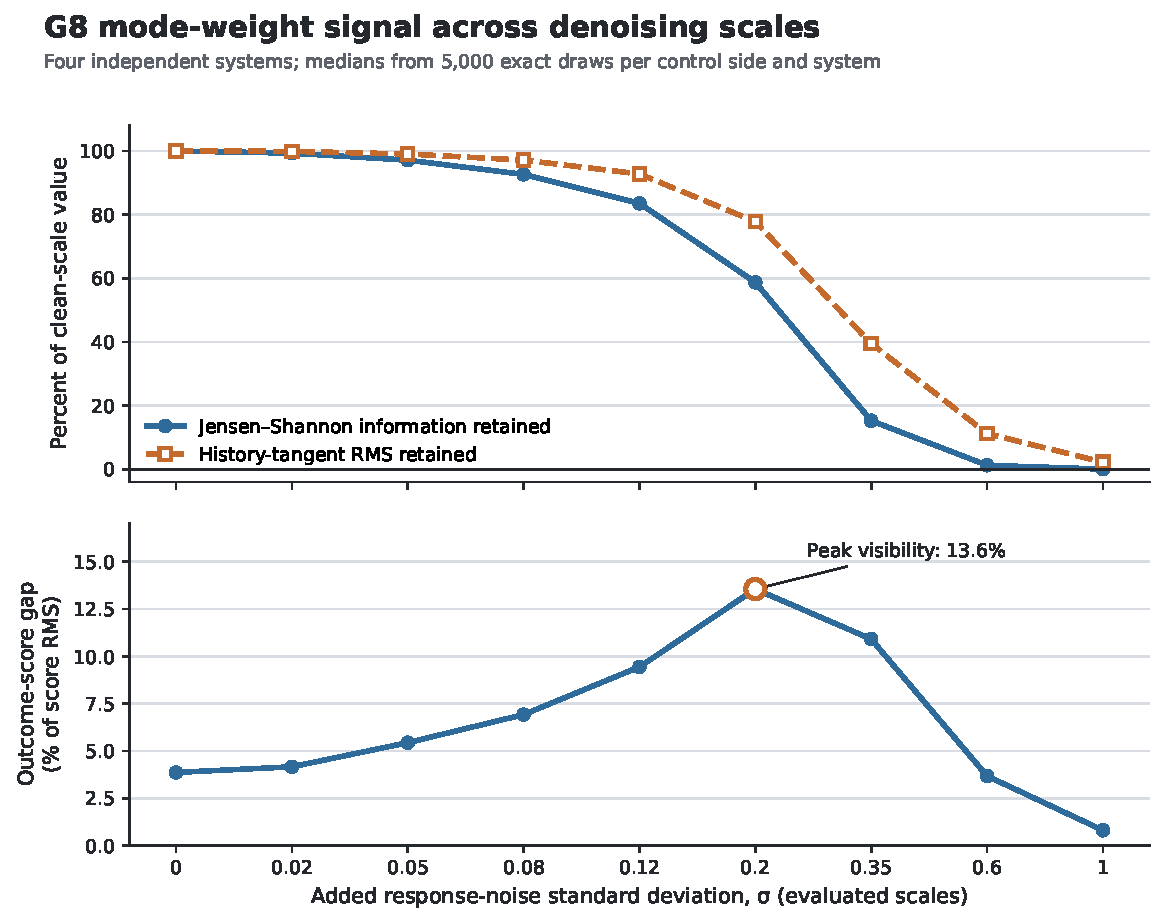
\includegraphics[width=\linewidth]{../../analysis/g8_score_visibility_audit_2026-07-13/g8_score_visibility.pdf}
\caption{Oracle visibility of the G8 mode-weight contrast across denoising
scales.  Top: finite law information and history-tangent magnitude, normalized
to the clean scale.  Bottom: separation between the two conditional outcome
scores relative to their RMS magnitude.  Points are medians over four independent
systems; each system uses 5,000 exact draws per control side.}
\label{fig:g8-score-visibility}
\end{figure}

The contrast itself is nevertheless learnable.  A separate balanced-classification
experiment trains directly on 4,000 responses per control side, tunes on 1,000,
and evaluates on 10,000 held-out responses per side.  It crosses four independent
G8 systems and two data seeds per system.  No classifier receives the control
label as an input.  With equal class priors, its probability estimate is converted
to the exact bounded finite witness $(2\widehat\eta-1)/\delta$ and then integrated
against the quartic readout.

\begin{center}
\begin{tabular}{@{}lrrr@{}}
\toprule
Estimator & AUC & Witness NRMSE & Median effect error \\
\midrule
Bayes witness & 0.768 & 0.000 & 0.33\% \\
empirical typed difference & --- & --- & 0.70\% \\
MLP on motif coordinates & 0.768 & 0.229 & 1.13\% \\
typed quartic logistic & 0.768 & 0.372 & 1.16\% \\
fourth-order polynomial logistic & 0.768 & 0.346 & 2.24\% \\
MLP on raw path and baseline history & 0.763 & 0.421 & 3.05\% \\
quadratic motif logistic & 0.508 & 1.002 & 99.64\% \\
linear motif logistic & 0.499 & 1.000 & 100.00\% \\
\bottomrule
\end{tabular}
\end{center}

This is the cleanest positive result in the new suite.  The flexible contrast
classifier reaches Bayes AUC and accurately recovers the typed effect; the raw
32-dimensional path model does nearly as well without the oracle motif basis.
Linear and quadratic routes stay at chance and reproduce the exact negative
controls.  Full witness recovery remains harder than one projected functional---the
motif MLP has witness NRMSE 0.229 despite only 1.13\% typed-effect error---which is
direct evidence for typed projection rather than unnecessary reconstruction of
the entire law derivative.

The exact first/second-moment Gaussian shadow supplies the mandatory confusion
control.  Across the same four system seeds and two data seeds, the raw
path/history classifier has median AUC 0.499 (range 0.496--0.505).  Its absolute
projected quartic effect is below 0.16\% of the matched positive G8 effect in every
cell.  Thus neither a low-order mismatch nor accidental inclusion of the control
label explains the positive G8 result.

This panel is developmental, not confirmatory: it has only four independent
systems, uses clean histories, and studies the supported $-1$ versus $+1$
contrast.  The motif and quartic variants use oracle centering/basis information;
the raw path/history MLP is the relevant representation-agnostic comparator.  Its
10,000-draw evaluation is larger than the sampler audit, although plug-in standard
errors projected to 512 draws per side are still only 2.0\% of truth for the
motif MLP and 2.4\% for the raw model.  A final common-budget replication remains
required.

A frozen-generator repair experiment then samples each fitted G8 control-zero
midpoint law and reweights those draws with the same raw path/history classifier.
It crosses two independent systems, two data seeds, two model seeds, and five
generator families.  The exact midpoint law with the learned classifier reaches
median NRMSE 0.125 and slope 0.889; replacing the learned classifier by the Bayes
posterior reaches NRMSE 0.013 and slope 1.001.  Thus the reweighting identity and
Monte Carlo procedure are numerically valid.

\begin{center}
\begin{tabular}{@{}lrrrr@{}}
\toprule
Frozen proposal law & Raw NRMSE & Raw slope & Guided NRMSE & Guided slope \\
\midrule
EDM & 0.991 & 0.010 & 0.602 & 0.398 \\
flow matching & 0.992 & 0.009 & 0.648 & 0.353 \\
affine flow & 0.945 & 0.055 & 0.661 & 0.340 \\
autoregressive MDN & 0.941 & 0.060 & 0.669 & 0.332 \\
autoregressive Transformer & 0.996 & 0.005 & 0.737 & 0.264 \\
\bottomrule
\end{tabular}
\end{center}

All 44 records, including four oracle-midpoint controls, completed successfully.
Median guided effective sample fractions are 0.83--0.84 and classifier
probabilities almost never saturate, so importance degeneracy is not the failure.
Guidance recovers a real fraction of the missing mass effect for every proposal
law, but none approaches the exact-midpoint control.  In the error decomposition
of the main text, the contrast head is useful while the $Q$-versus-$M$ geometry
term remains large.  This rejects both extreme explanations: the generator is not
irrelevant, and a classifier head alone is not a complete generative repair.

An 80-cell endpoint-expert factorial tests the complementary repair: enforce the
global gate first, then fit a separate full-law expert to each supported endpoint.
The total budget remains 8,000 rows (4,000 per expert), the declared control is
removed from expert inputs, and the gate deterministically selects the $-1/+1$
expert.  It crosses four systems, two data seeds, two model seeds, and five
backends; every cell succeeds.

\begin{center}
\begin{tabular}{@{}lrrr@{}}
\toprule
Endpoint expert & Fair energy & Quartic NRMSE & Quartic slope \\
\midrule
EDM & 0.704 & 0.665 & 0.336 \\
affine flow & 0.704 & 0.750 & 0.251 \\
autoregressive MDN & 0.714 & 0.823 & 0.179 \\
flow matching & 0.703 & 0.965 & 0.035 \\
Gaussian NLL & 0.718 & 1.000 & 0.000 \\
\bottomrule
\end{tabular}
\end{center}

Compared with shared balanced-control fits, explicit experts materially improve
EDM (slope 0.013 to 0.336), affine flow (0.046 to 0.251), MDN (0.095 to 0.179),
and flow matching (0.001 to 0.035).  Yet they remain far below the direct finite
classifier.  This is the strongest architectural diagnosis in the suite: weak
conditioning is one failure, while a full-law expert objective that underweights
the fourth-order topology is another.  A normalized gate is necessary here but
not sufficient.

The frozen-anchor stochastic-interpolant factorial supplies a separate transport
control.  It reuses the exact core splits and Gaussian anchors, changes only
$\beta_t=t$ versus $t^2$, fixes diffusion amplitude one, and crosses the same two
systems, two data seeds, and two model seeds on G1 and G8.  All 32 fits succeeded.

\begin{center}
\begin{tabular}{@{}llrrr@{}}
\toprule
Law & Schedule & Fair energy & Typed NRMSE & Typed slope \\
\midrule
G1 Gaussian location & linear & 1.513 & 0.338 & 0.908 \\
G1 Gaussian location & squared & 1.513 & 0.319 & 0.864 \\
G8 fourth-order path & linear & 0.717 & 0.993 & 0.0075 \\
G8 fourth-order path & squared & 0.710 & 0.999 & 0.0007 \\
\bottomrule
\end{tabular}
\end{center}

Typed columns use the G1 finite mean effect and the supported G8 quartic effect at
$\delta=1$.  The 64/128/256-step G8 slopes agree to within about one percentage
point.  Squared $\beta$ improves G8 fair energy but worsens the SID channel, while
both schedules learn a nontrivial G1 mean effect.  This is direct evidence against
the two most convenient optimization explanations: the sampler is stable, and
removing the initial response impulse does not expose the missing mass derivative.

Finally, an exact-density permutation audit removes sampling and quartic-readout
noise.  It measures the held-out log-density gain from supplying the correct
shape control instead of a permuted control.  The oracle gain is median 0.274
nats.  The autoregressive MDN retains 19.4\% of it, affine flow 12.4\%, and the
autoregressive Transformer only 2.9\%; Gaussian NLL and Gaussian DSM retain zero.
Thus the attenuation is already present in the fitted conditional density and is
not created by the sampler or the fourth-order statistic.
